\documentclass[12pt, A4, titlepage]{article}
\usepackage[utf8]{inputenc}
\usepackage{lipsum}
\usepackage{setspace}
\usepackage{hyperref}
\usepackage{anyfontsize}
\usepackage{enumitem}
\usepackage{minted}
\usepackage{graphicx}
\usepackage[inkscapearea=page]{svg}

\newcommand\HHUGE{\fontsize{50pt}{18pt}\selectfont}
\newcommand\TitleFont{\fontsize{25pt}{15pt}\selectfont}
\setminted[python]{breaklines, framesep=2mm, fontsize=\footnotesize, numbersep=5pt}


\title{\vspace{-2cm} \HHUGE{Project 1} \\ \vspace{1cm} \TitleFont{Movie Database} \\ \vspace{0.7cm} \LARGE CmpE 321, Introductin to Database Systems, Spring 2023 \vspace{6cm}}
\author{
    Simar Ahmet Kahya - 2020400378 \\
    Bahadır Gezer - 2020400039 \\
}
\date{2 April 2023}

% \doublespacing
\onehalfspacing
% \singlespacing
\begin{document}

\maketitle

\newpage
\tableofcontents

\newpage
\section{Introduction}

\indent \indent The objective of this project is to design a database system for movies. The system will allow users to reserve seats for movie screenings, and also provide a rating mechanism for movies. The project will follow the standard database design process, including conceptual and logical design, as taught in class.

\section{Conceptual Database Design}

\indent \indent The first step in designing the database system for movies is to perform the conceptual database design, also known as the entity-relationship (ER) design. This process involves drawing ER diagrams to capture all the information, following the approach described in the lectures. The goal of the ER design is to identify all the entity sets and relationship sets in a reasonable way, taking into account the given information and constraints as much as possible. \\

We start by identifying the entities. Our diagram has User, Audience, Director, Rating Platform, Movie, Movie Session, Genre, Theater, and Database Manager as entities. These entities hold the attributes given in the project description. \\

We then have to decide on the relations between these entities. We had long discussions about the use of aggregation, ternary relationship and maybe even weak entities, but in the end decided on a simpler approach on the ER diagram. This gives more flexibility and ease-of-use in the actual database. \\

The first, and very obvious, relationship is the ISA relationship between the User, Audience, and Director entities. In this system, every user is either a Director or an Audience. Both entities share the username, password, name, and surname attributes and use username as their primary key. The Director entity has an additional nation attribute. We decided the nation information can be an attribute and should be not null to satisfy the constraint. \\

Next, we have the relations for Rating Platform. The Rating Platform entity has two attributes, platform id and a name. These should both be unique, and the platform id is used as a primary key to connect with Audience and Director entities. Each Audience can subscribe to a Rating Platform and each Director is on at most one Rating Platform. A Rating Platform can hold many Director and Audience entities. \\

Movie entity has two relations, just like the Rating Platform, with Audience and Director; which are Rate, and Directed, respectively. Each Movie can be rated by an Audience, and each Audience can rate multiple Movies. The Rate relation has a descriptive attribute, rating. Which allows us to find a rating uniquely by using movie id and audience username. This relation is not connected to the Ticket relation or Rating Platform. We've tried this and iterated over many designs, and went for a flexible solution in the end. This solution also allows us to uniquely identify ratings just with username and movie id. Other solutions involving aggregation with Rating Platform involving this property. The second relation on movie is between the Director. Each movie must have one Director directing it. Directors can direct multiple Movies. Other constraints regarding Movie, Director, Rating Platform, and Rate are not included in the ER, following our simple and flexible ER design pattern. These constraints can be fulfilled in the actual database creation phase. \\

The Sequence relation is used to keep track succession of movies. One hand of it the predecessor and the other is, logically the successor movie. This many-to-many relation can be used for checking if the audience has tickets to movie sessions of predecessor movies. \\

Movie Session is separated from the Movie entity. These two entities are connected with a relation. This separation somewhat allows flexibility in the ER design, but it is mostly about removing duplicate data. We can have one copy of Movie details by separating Movie from Movie Session, each Movie Session at least and at most one Movie, and each Movie can have multiple Movie Sessions. This is captured by the Showing relation. \\

Movie session has a relation that holds information about ticket purchases. This relation is with the Audience entity, which does the purchasing. The ticket information is held with a many-to-many mapping between Audience and Movie Session entities. This relation is necessary to check when the Audience wants to rate a movie. "An audience can only rate a movie if it bought tickets to a movie session which screens the movie." this sentence has 3 entities and 3 relations in it. We did not use aggregation, or even double aggregation to connect these entities and relations. This would add unnecessary complexity and rigidness to the database. These checks can be done implicitly with conditions when creating tables. The ER diagram just provides the necessary foundation for these checks. \\

The Movie Session entity has another relation, Screening. This relation is between Movie Session and Theater. The Theater entity hold information related to a Theater. We remove duplicate data by holding theater information not inside the movie session entity but in another entity. Then we can only hold the mapping information between movie session and theater information for that movie session.  Each Movie Session must have one and only one Theater. Each Theater can hold multiple Movie Sessions. \\

Lastly, we have the Category relation between Genre and Movie. Each Genre has a genre id and a name. Both of which are unique, and genre id is used as the primary key. Each movie has at least one Genre and each genre can be associated with many Movie entities. \\

\section{Logical Database Design}

\indent \indent The second part of the project involves converting the ER diagrams created in the first part into relational tables, based on a set of simple rules as described in the textbook and lectures. This process is known as the logical database design and will result in a set of tables that accurately represent the information and constraints captured in the ER diagrams.\\

To complete this part of the project, we started by analyzing each entity set and relationship set in the ER diagrams and identifying the corresponding relations in the relational model. For each relation, we provided a schema that includes the relation name, attribute names, and attribute domains. The schema we've created are as follows: \\

\begin{itemize}
    \item Audience(username: string, password: string, name: string, surname: string)
    \item Genre(id: integer, name: string)
    \item Database\_Managers(username: string, password: string)
    \item Rating\_Platform(id: integer, name: string)
    \item Theater(id: integer, name: string, capacity: integer, district: string)
    \item Director(username: string, password: string, name: string, surname: string, nation: string)
    \item Movie(id: integer, name: string, duration: integer, overall\_rating: real, director\_name: string)
    \item Movie\_Session(id: integer, movie\_id: integer, theater\_id: integer, time\_slot: integer, date: string)
    \item Ticket(username: string, session\_id: integer)
    \item Platform\_Subscription(username: string, platform\_id: integer)
    \item Movie\_Ratings(username: string, rating: real, movie\_id: integer)
    \item Movie\_Genre(movie\_id: integer, genre\_id: integer)
    \item Movie\_Predecessor(predecessor\_id: integer, successor\_id: integer)
\end{itemize}

\section{SQL DDL Statements}

\indent \indent In the third and final part of the project, we implemented the database and application program based on the conceptual and logical database designs created in parts 1 and 2. The first step in this process was to write SQL DDL statements that create the tables we designed in part 2. \\

We started by creating a new database in MySQL and then executed the createTables.sql script, which contained all the SQL DDL statements necessary to create the tables we designed. Each table had the appropriate constraints, including primary keys, foreign keys, unique constraints, and NOT NULL constraints. We also added comments to the script to make it easier to understand. The SQL files are included in the appendix. The comments did not fit in the page, the source code is also included as separate files. 

\appendix

\section{ER Diagram}
% \rotatebox{270}{\includesvg[scale=0.6]{pictures/er.svg}}
\hspace*{-1.5cm}\rotatebox{270}{\hspace*{-4cm}\vspace*{5cm}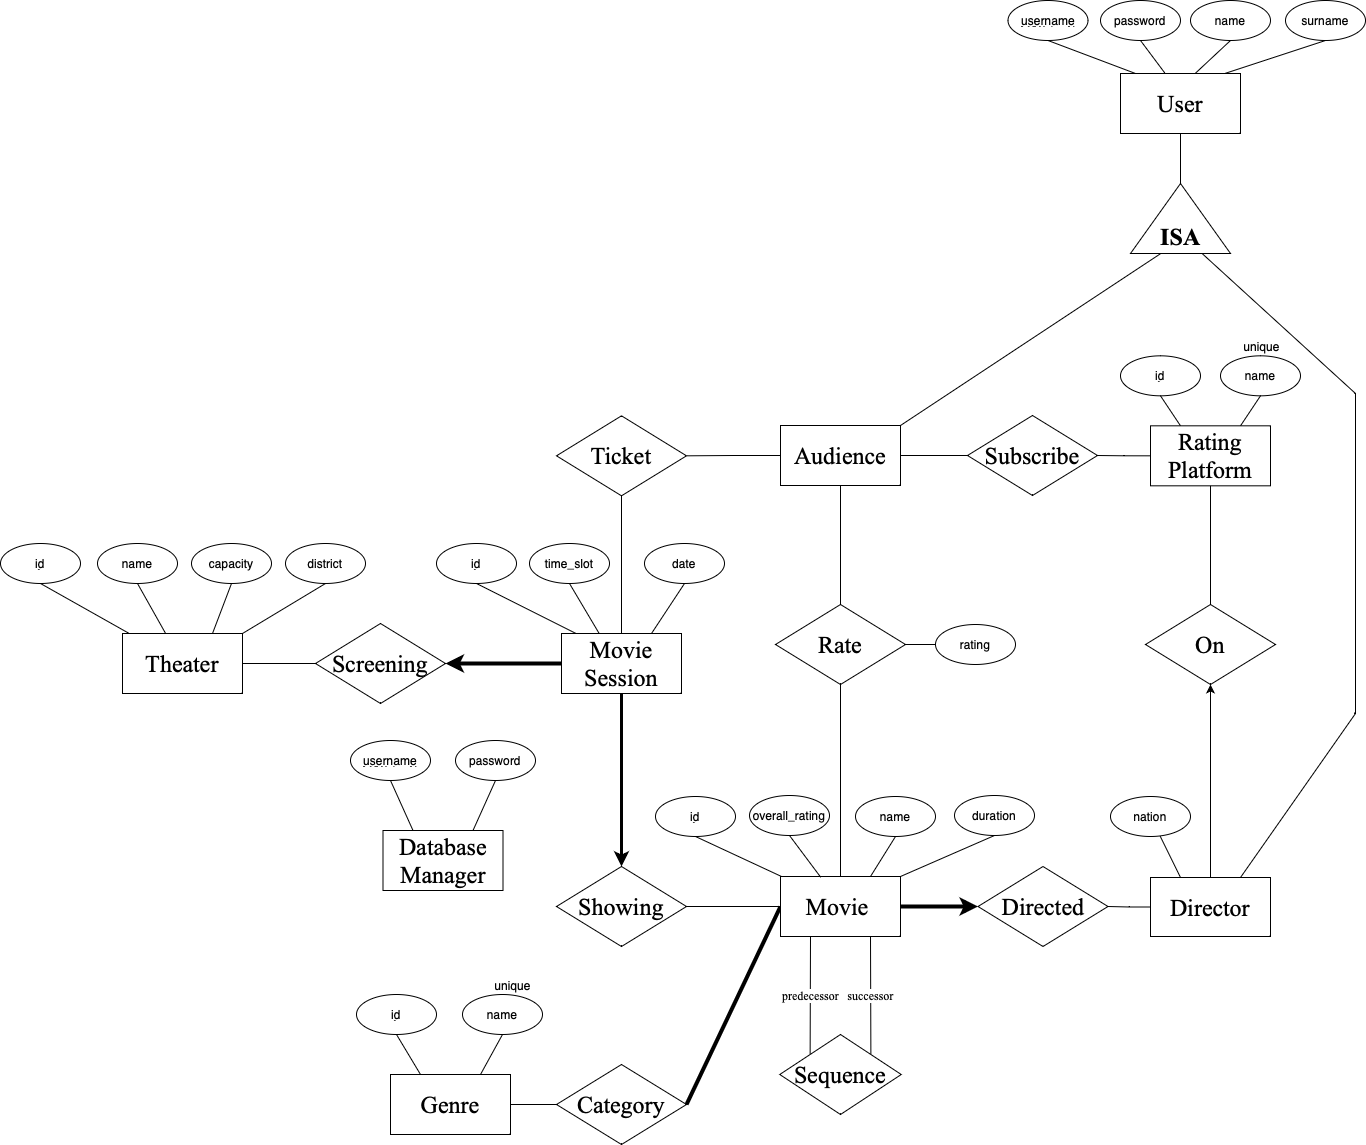
\includegraphics[scale=0.45]{pictures/er.drawio.png}}

\newpage
\section{SQL Source Code}

\subsection{createTables.sql}
\begin{minted}{sql}
CREATE TABLE Audience (
    username VARCHAR(255),
    password VARCHAR(255) NOT NULL, -- every user requires a password
    name VARCHAR(255),
    surname VARCHAR(255),
    PRIMARY KEY (username)
);
CREATE TABLE Genre (
    id INT,
    name VARCHAR(255) UNIQUE, -- from description
    PRIMARY KEY (id)
);
CREATE TABLE Database_Managers (
    username VARCHAR(255),
    password VARCHAR(255),
    PRIMARY KEY (username)
);
CREATE TABLE Rating_Platform (
    id INT,
    name VARCHAR(255) UNIQUE, -- from description
    PRIMARY KEY (id)
);
CREATE TABLE Theater (
    id INT,
    name VARCHAR(255),
    capacity INT,
    district VARCHAR(255),
    PRIMARY KEY (id)
);
CREATE TABLE Director (
    username VARCHAR(255),
    password VARCHAR(255) NOT NULL, -- every user requires a password
    name VARCHAR(255),
    surname VARCHAR(255),
    nation VARCHAR(255) NOT NULL, -- every director must have only one nation
    platform_id INT,
    PRIMARY KEY (username),
    FOREIGN KEY (platform_id)
        REFERENCES Rating_Platform (id)
        ON DELETE SET NULL ON UPDATE CASCADE -- director *can* have a platform
);
CREATE TABLE Movie (
    id INT,
    name VARCHAR(255),
    duration INT,
    overall_rating REAL,
    director_name VARCHAR(255) NOT NULL,
    PRIMARY KEY (id),
    FOREIGN KEY (director_name)
        REFERENCES Director (username)
        ON DELETE CASCADE ON UPDATE CASCADE -- every movie requires a director
);
CREATE TABLE Movie_Session (
    id INT,
    movie_id INT NOT NULL,
    theater_id INT NOT NULL,
    time_slot INT NOT NULL, -- movie sessions must have a time and date
    date DATE NOT NULL,
    PRIMARY KEY (id),
    FOREIGN KEY (movie_id)
        REFERENCES Movie (id)
        ON DELETE CASCADE ON UPDATE CASCADE, -- every movie session requires a movie
    FOREIGN KEY (theater_id)
        REFERENCES Theater (id)
        ON DELETE CASCADE ON UPDATE CASCADE -- every movie session requires a theater
);
CREATE TABLE Ticket (
    username VARCHAR(255),
    session_id INT,
    PRIMARY KEY (username , session_id),
    FOREIGN KEY (username)
        REFERENCES Audience (username)
        ON DELETE CASCADE ON UPDATE CASCADE, -- every ticket must have an audience
    FOREIGN KEY (session_id)
        REFERENCES Movie_Session (id)
        ON DELETE CASCADE ON UPDATE CASCADE -- every ticket must have a movie session 
);
CREATE TABLE Platform_Subscription (
    username VARCHAR(255),
    platform_id INT,
    PRIMARY KEY (username , platform_id),
    FOREIGN KEY (username)
        REFERENCES Audience (username)
        ON DELETE CASCADE ON UPDATE CASCADE, -- every subscription must have an audience
    FOREIGN KEY (platform_id)
        REFERENCES Rating_Platform (id)
        ON DELETE CASCADE ON UPDATE CASCADE -- every subscription must be on a platform
);
CREATE TABLE Movie_Ratings (
    username VARCHAR(255),
    movie_id INT,
    rating REAL,
    PRIMARY KEY (username , movie_id),
    FOREIGN KEY (username)
        REFERENCES Audience (username)
        ON DELETE CASCADE ON UPDATE CASCADE, -- every rating must have an audience connected to it
    FOREIGN KEY (movie_id)
        REFERENCES Movie (id)
        ON DELETE CASCADE ON UPDATE CASCADE -- every rating requires a movie
);
CREATE TABLE Movie_Genre (
    movie_id INT,
    genre_id INT,
    PRIMARY KEY (movie_id , genre_id),
    FOREIGN KEY (movie_id)
        REFERENCES Movie (id)
        ON DELETE CASCADE ON UPDATE CASCADE, -- every genre-movie mapping must have both a genre and a movie
    FOREIGN KEY (genre_id)
        REFERENCES Genre (id)
        ON DELETE CASCADE ON UPDATE CASCADE
);
CREATE TABLE Movie_Predecessor (
    predecessor_id INT,
    successor_id INT,
    PRIMARY KEY (predecessor_id , successor_id),
    FOREIGN KEY (predecessor_id)
        REFERENCES Movie (id)
        ON DELETE CASCADE ON UPDATE CASCADE, -- every movie-movie mapping must have both movies 
    FOREIGN KEY (successor_id)
        REFERENCES Movie (id)
        ON DELETE CASCADE ON UPDATE CASCADE
);
\end{minted}

\subsection{dropTables.sql}
\begin{minted}{sql}
DROP TABLE Movie_Predecessor;
DROP TABLE Movie_Genre;
DROP TABLE Movie_Ratings;
DROP TABLE Platform_Subscription;
DROP TABLE Ticket;
DROP TABLE Movie_Session;
DROP TABLE Movie;
DROP TABLE Director;
DROP TABLE Theater;
DROP TABLE Rating_Platform;
DROP TABLE Database_Managers;
DROP TABLE Genre;
DROP TABLE Audience;
\end{minted}

\end{document}
